\documentclass[10pt,journal]{IEEEtran}
\usepackage{cite, graphicx, subfigure, amsmath} 
\usepackage{algorithm, algorithmic}
\usepackage{graphicx}
\usepackage{mdwlist}
\usepackage{float}
\usepackage{url}
\interdisplaylinepenalty=2500

% *** Do not adjust lengths that control margins, column widths, etc. ***
% *** Do not use packages that alter fonts (such as pslatex).         ***
% There should be no need to do such things with IEEEtran.cls V1.6 and later.


\begin{document}
% paper title
\title{Parallelizing k-means for Image Segmentation}


% author names and IEEE memberships
% note positions of commas and nonbreaking spaces ( ~ ) LaTeX will not break
% a structure at a ~ so this keeps an author's name from being broken across
% two lines.
% use \thanks{} to gain access to the first footnote area
% a separate \thanks must be used for each paragraph as LaTeX2e's \thanks
% was not built to handle multiple paragraphs
\author{Chris Jordan,
Victor Janmey,
and Raymond W. Ko}% <-this % stops a space


% The paper headers
%\markboth{<+Journal of VIM-\LaTeX\ Class Files,~Vol.~1, No.~8,~August~2002+>}{
%<+Bhardwaj \MakeLowercase{\textit{et al.}+>}: <+Skeleton of IEEEtran.cls for Journals in VIM-Latex+>}
% The only time the second header will appear is for the odd numbered pages
% after the title page when using the twoside option.


% If you want to put a publisher's ID mark on the page
% (can leave text blank if you just want to see how the
% text height on the first page will be reduced by IEEE)
%\pubid{0000--0000/00\$00.00~\copyright~2002 IEEE}


% use only for invited papers
%\specialpapernotice{(Invited Paper)}


% make the title area
\maketitle

\begin{abstract}
Abstract goes where? Abstract goes here!
\end{abstract}

\begin{keywords}
k-means, k-means++, parallel programming, triangle inequality
\end{keywords}

\section{Introduction}
\PARstart{T}{he} k-means algorithm performs a simple grouping of particles into a fixed number of clusters.
It has an vast amount of uses in fields such as
machine learning, computer vision, and network analysis.

In the case of machine learning, it is useful in unsupervised learning methods, 
dividing data for more specific classifiers, and the selection of of examples for k-nearest neighbors.

For computer vision, one frequent task is to segment images using the difference in pixel intensity as a distance
metric. One can then use the k-means algorithm to estimate object boundaries, or use it as a cue for other algorithms
that perform object recognition.

Additionally, the use of k-means is not limited only to images. In network analysis it can be used to find communities.

However, in this paper, we will focus on the problem of image segmentation, towards which we will try to tune the code
to run as fast as possible.

\section{Analysis of Algorithm}
Before focusing on the actual implementation, the k-means algorithm
was examined to see what sections could be effectively parallelized.

\subsection{\textit{k-means}}
The k-means algorithm basically consists of three steps:
choosing $k$ initial clusters, an assignment step, and an
update step. In the assignment step, particles get assigned
to clusters. In the update step, the new mean of a cluster
is recomputed by taking the average of all the values
of the particles in that cluster.

\begin{algorithm}
\caption{naive k-means algorithm}
\begin{algorithmic}[1]
\STATE{choose $k$ initial means as centers}
\FOR{each particle $p$}
    \FOR{each mean $k$}
        \STATE{calculate distance from $p$ to $k$}
        \IF {distance $<$ previous calculated distance}
            \STATE{mark down mean}
        \ENDIF
    \ENDFOR
    \STATE{put $k$ into last marked down cluster with mean}
\ENDFOR
\FOR{each cluster $c$}
    \STATE{sum $\leftarrow$ 0}
    \FOR{each particle $p$ in $c$}
        \STATE{sum $\leftarrow$ sum $+$ p}
    \ENDFOR
    \STATE{new mean of cluster $c$ $\leftarrow$ sum / $|c|$}
\ENDFOR
\STATE{repeat steps 2 to 17 until new means converge and no longer change}
\end{algorithmic}
\end{algorithm}

An initial cursory glance at the algorithm indicates that there are parts that are
easy to parallelize.

The initial steps for choosing $k$ can be done in any fashion, and since they are not
dependent on each other, can simply be randomly chosen in parallel.

The second step, the assignment step, is the time dominating factor in the calculation since
it is $O(kn)$ due to the fact that for every particle, each of the $k$-clusters must be considered.
Nevertheless, since the inner for loop and assignment is independent of every other iteration,
it is an example of ``embarrassingly'' parallel programming, and as such using a \emph{parallel for}
loop construct is enough to evenly distribute the work between $n$ processors.

For the third step, the update step, a \emph{parallel reduce} was used to sum up the values of the particles
before performing a division to determine the mean. While it is also possible to use a \emph{parallel for} construct
over the outer for loop, it does not scale well if $k$ is smaller than the number of processors.
A \emph{parallel reduce} would almost always utilize the processors fully since the number of particles usually
outnumbers the number of processors.

\subsection{k-means++}
While the runtime of the original algorithm where the initial \textit{k}-clusters are randomly chosen is acceptable
, it has been shown that the worst case running time
can be super-polynomial \cite{slow}. By using the k-means++ algorithm to choose the initial
starting clusters, the algorithm is guaranteed a solution that is within a factor of $O(log k)$
to the optimal k-means solution.

The fundamental idea of the k-means++ algorithm is to prevent clusters from being too close together
by spreading out the assignment of clusters.

\begin{algorithm}
\caption{k-means++ algorithm}
\begin{algorithmic}[1]
\STATE{choose one center at random among the data points}
\FOR{each data point $x$}
    \STATE{compute D(x), the distance between $x$ and the nearest center already chosen}
\ENDFOR
\STATE{add one data point as a cluster, using a weighted probability distribution where a point $x$ is chosen with probability proportional to D$(x)^2$}
\STATE{repeat steps 2 to 5 until $k$ centers have been chosen}
\STATE{run standard k-means clustering algorithm}
\end{algorithmic}
\end{algorithm}

Similar to the naive k-means algorithm, the time dominant step for k-means++ is the first step
since for every particle, an iteration must be performed for every cluster. Since the computations of
finding which cluster has the minimum distance to a given particle are independent of one another,
a \emph{parallel for} loop would suffice in efficiently parallelizing this section of the code.

The second part of the algorithm, which involves a prefix sum over an
array of shortest distances to a known center, can be implemented as a parallel prefix scan.

\section{Implementation}

In order to implement parallelization in the k-means program, we chose
Intel's Threading Building Block (TBB) framework since all the necessary parallel constructs
desired are present. TBB removes the need for the programmer to be concerned with
low-level thread management since this is automatically managed by a scheduler.
The only variable in the TBB implementation that we wish to tune is the grain size for the \emph{parallel\_for}
construct, since this has an effect on the total run time.

Because of the decision to use TBB, the C++ programming language had to be chosen instead of C, since
the interface to TBB constructs is a body class. Although class overhead is probably minimal,
C++ class constructors and destructors may contribute slightly to the runtime over a parallel implementation in C.

In addition to using TBB, we also decided to implement k-means using OpenMP as a baseline for comparison.
Determining whether TBB possessed some form of overhead was an important goal, and since OpenMP is
implemented in every major C/C++ compiler, it would also be interesting what sort of performance one could
get without using a specialized library.

In order to determine the effectiveness of parallelization, several experiments regarding
grain size, particle size, core size, and cluster size were run. Determining the optimal grain size
is important since an improper grain size may create unnecessary tasks (if too small) or be unable
to fully utilize the total number of cores (if too large). Particle size is also important since
it has implications towards what image resolutions today's technology can process at a reasonable speed.
If a certain response time is desired of a machine vision program, it might become necessary
to down-sample images received. Another aspect of interest regarding this algorithm is the
number of processors. At what point would we start seeing the benefits of parallelization?
Would we expect a linear speedup on an infinite number of processors? Finally, we would like
to answer the question of what an efficient cluster size would be. If an image has too many objects that need
to be segmented, would the algorithm become unusable? What about too few objects?

\section{Results}

In this section, all graphs are normalized to the fastest serial version, unless mentioned otherwise.
The fastest serial version was compiled with GCC version 4.3.2 with maximum optimization (-O3) and loops
unrolled (-funroll-all-loops). Additionally, cluster size is held constant at $k=50$ for all experiments
except the final experiment where optimal cluster size is determined.

All runtime experiments were performed on the SEAS acgrid30 - acgrid32 4-core Core2 x86 cluster machines, unless mentioned otherwise.
The machines we chose have 4 distinct cores that can run up to 4 hardware threads at a time. The image that we chose was
of the town of Porto Moniz with a resolution of $1280 \times 800$ pixels. This equates to
1,024,000 pixels.

\begin{figure}[htp]
\centering
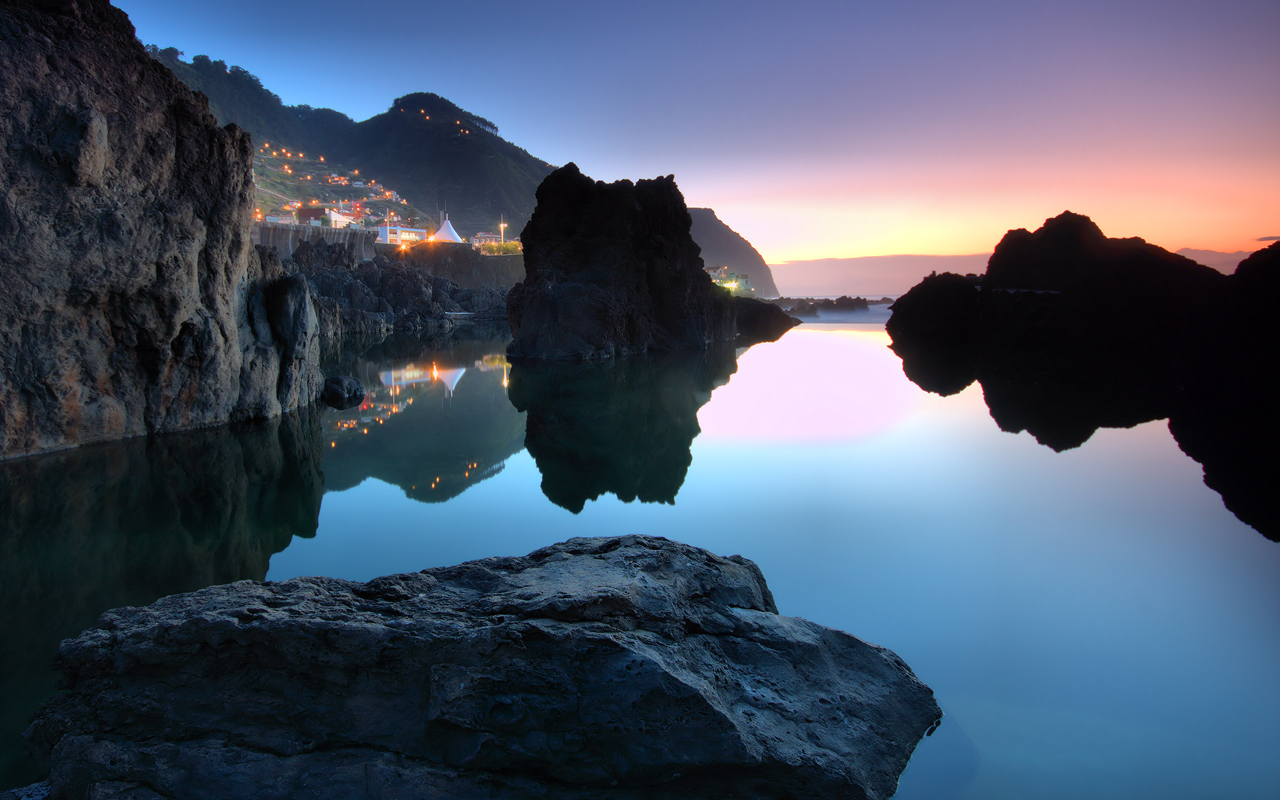
\includegraphics[width=.90\linewidth,bb=0 0 1280 800]{portomoniz.jpg}
\caption{The town of Porto Moniz}
\end{figure}

\subsection{Speedup vs. Grain Size}

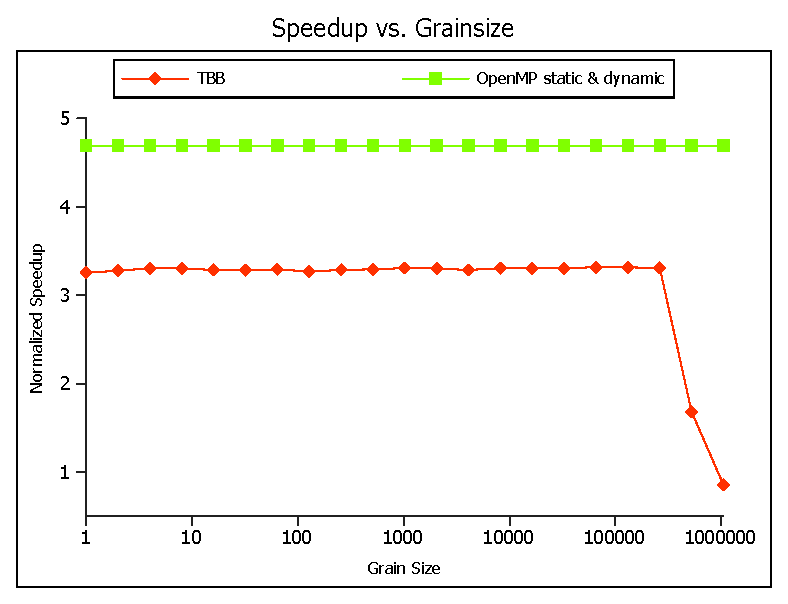
\includegraphics[width=.90\linewidth]{graph_grainsize}

As expected, TBB produces a somewhat ideal speedup until the grain size became too large to be evenly
distributed over the number of cores. Surprisingly, OpenMP exhibits super-linear speedup
with the static and dynamic scheduler. Either the grainsize configuration did not work, or
static values were pre-chosen, since varying grain size did not significantly affect grainsize.

\subsection{Speedup vs. Number of Particles}

In this experiment, we scaled the above image to vary the number of particles.

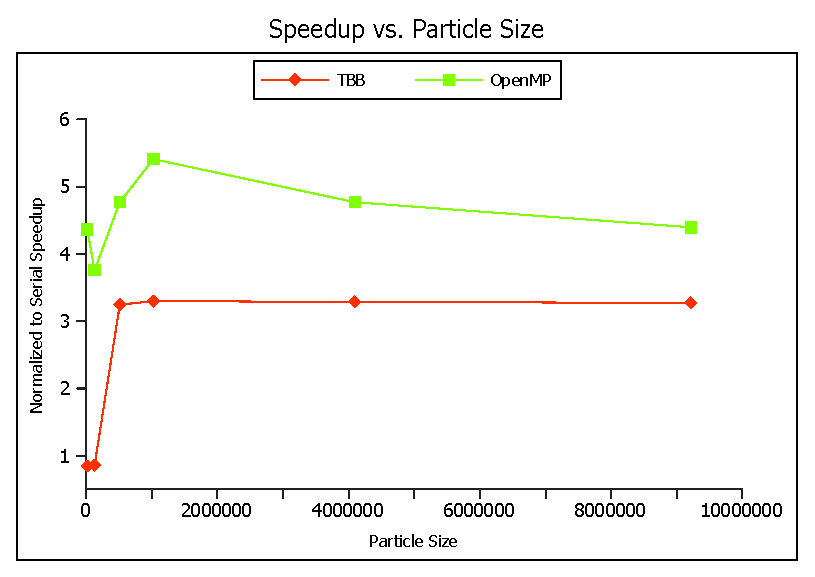
\includegraphics[width=.90\linewidth]{graph_speedup_vs_particle_size}

When the speedup is compared to the particle size, a particle size that is
too small results in a sub-optimal speedup. However, as the particle size
gets larger to more reasonable values, the speedup remains fairly linear for
TBB while the speedup for OpenMP decreases from the maximum theoretical linear speedup.

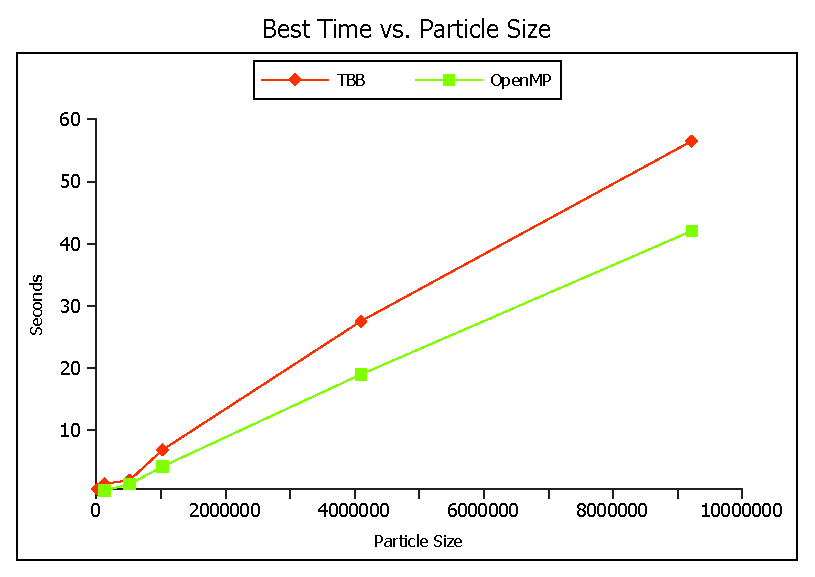
\includegraphics[width=.90\linewidth]{graph_best_time_vs_particle_size}

Since all the previous graphs were in terms of normalized speedups,
this graph was included to give a sense of runtimes on four cores.
This graph shows that run-time linearly scales with particle size with
OpenMP again producing better results.

\subsection{Speedup vs. Number of Cores}

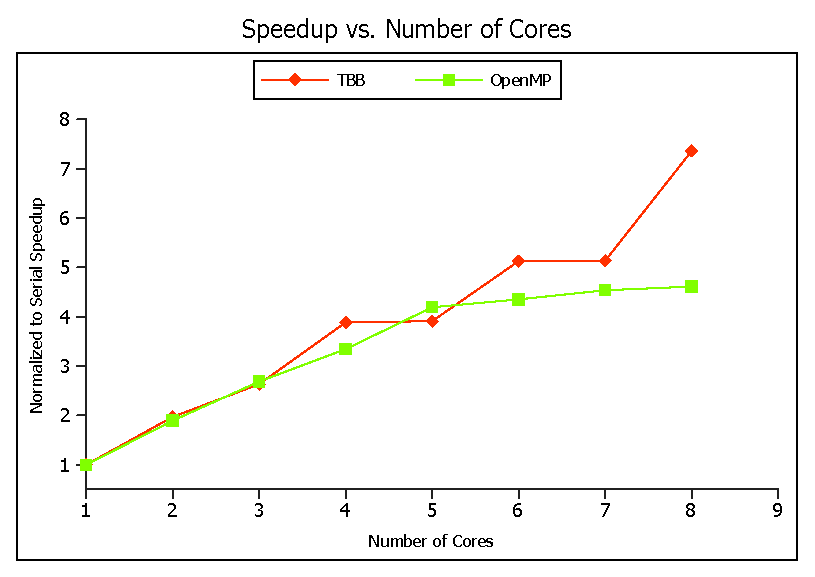
\includegraphics[width=.90\linewidth]{graph_cores}

Experimentation shows that TBB scales fairly linearly with the number of cores,
achieving a near linear speedup. However, OpenMP levels out at around 4.0, and shows
no further improvement.

\subsection{Speedup vs. Number of Clusters}

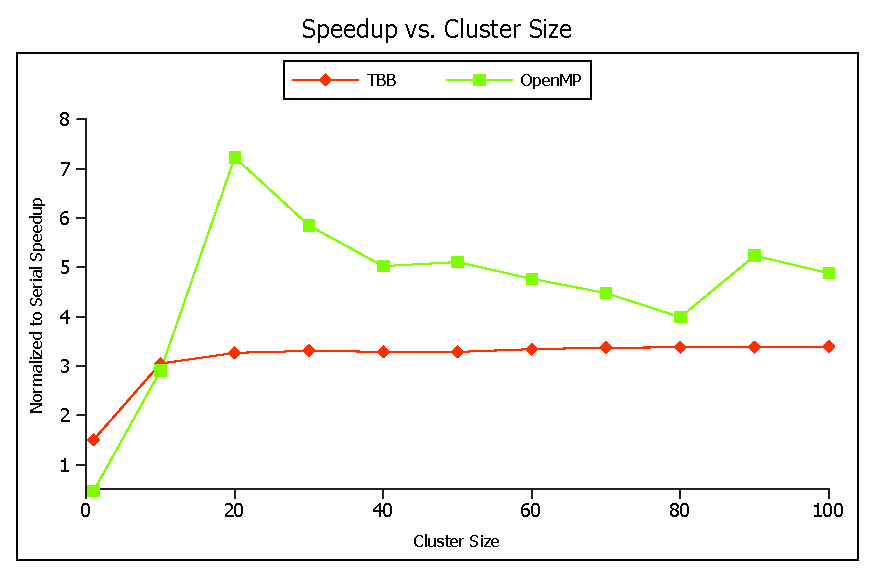
\includegraphics[width=.90\linewidth]{graph_clusters}

For TBB, speedup is fairly linear on four cores when compared to the serial version, except
for when values of $k$ are extremely small. Like the graphs, before OpenMP exhibits better
peformance than TBB in almost all cases.

\section{Discussion of Results}

\subsection{Speedup vs. Grain Size}
In the case of OpenMP, the speedup is independent of grain size until the grain size becomes so large
that the total number of particles divided by the grain size is larger than the number of cores present. It is surprising to note that with OpenMP  superlinear speedup is achieved.
We have several theories explaining the superlinear speedup. Initially it was thought that
loop unrolling might be the cause; however, the linear version also had the loop unrolling
compilation flag, so this possibility was eliminated. Upon brief inspection of the assembly
code in the GNU debugger (gdb), it was revealed that gcc made significant use of the
Intel Single Instruction Multiple Data (SIMD) instructions in a fashion that is more efficient than TBB.
A more detailed comparison of the assembly instructions between the two implementations would be very informative, but that is beyond the scope of this paper.
Finally, another hypothesis was that OpenMP better utlized the memory bus than TBB, either
by producing a sequence of instructions that read with more throughput or by producing a better
read-ahead effect. Cache size is believed to be strongly involved since our image
produces a \texttt{double} array of size $1024000 \textrm{ particles}
\times 8 \textrm{ bytes} \times 3 \textrm{ channels} = 23.4375$ MB, which is far larger than the L2 cache on the machines we tested.

\subsection{Speedup vs. Number of Particles}

Intel's TBB exhibit a stable, almost unvarying level of speedup after the particle size is large
enough to ensure that each of the cores has enough work distributed to it. The same is true
for OpenMP, where if the work is too small, speedup gains are not as efficient as they
can be. This seemingly reflects one of the basic rules of thumb in parallel programming:
if your data set is too small, it is better to fall back to the serial version instead of
creating the extra overhead of parallelization without gaining any benefit from it. Like
the above results for speedup vs. grain size, the OpenMP seems to get astonishing
superlinear speedups. Since this part of the experiment involves manipulating large sets
of data, the theory of better memory throughput or read-ahead effects seems to be supported
since read-ahead becomes much more apparent when the number of particles is small (resulting
in all of the particles being read into the L2 cache). As particle size increases, the effects
of read-ahead seem to level off, but memory throughput is still higher than with TBB. The
slope in performance as particle size increases seems to suggest that the theory that
the OpenMP code performs more FLOPs per second than the TBB code is not the right explanation
for the increased performance. Such a plot would be much more linear since the instructions would
consume a nearly constant number of FLOPs per particle.

As a side note, a comparison of runtime vs. particle size also shows a fairly linear speedup, meaning
that increasing the resolution only approximately increases the runtime of the parallel k-means
algorithm linearly. The resolution chosen for resolution, 1280x800, or 1,024,000 particles, takes 
approximately 4 seconds. Between 512,000 particles and 128,000 particles, it is possible to have sub-second
times. This means that NTSC DVD resolution pictures (720x480) can be processesed by the k-means algorithm
on four cores almost immediately, making it possibly suitable for use on realtime or interactive systems.

\subsection{Speedup vs. Number of Cores}

A noticable difference between the two implementations in this experiment is the fact that OpenMP starts to perform worse than TBB
as the number of cores increase. This provides further evidence for the memory throughput theory mentioned
in the previous experiments. Since this experiment was performed on a dual-socket quad-core, there is an
extra level of indirection that is present when the CPUs access the memory bus. As a result, it is
understandable that a decrease in the total memory throughput would cause the speedups to level off
However, this does not explain the results using Intel's TBB, which maintains a reasonably linear speedup.
It is possible that Intel's scheduler is tuned to better peform on dual-socket quad-core and not as well
on a dual-socket dual-core, which the rest of the experiments are run on. Since the scheduler is implemented
on a dynamically linked library, it is possible that future versions of the library will exhibit better performance.

Nevertheless, since TBB exhibits a reasonably linear speedup (7.0 on 8 cores), a linear regression fit (not shown),
optimistically shows a speedup of around 50.0 on 64 cores. Unfortunately, we do not possess dedicated machines
with this number of cores on which to run tests. We attempted to cross-compile our TBB code for the Niagara II SPARC machine we did have access to, however, this was not possible because of the TBB libraries. We can still predict that the effects on memory bandwith
and cache coherence from a many-core environment would be detrimental to runtime since this is not a read-many-times, write-once type of algorithm. Thus the actual speedup on a 64 core environment will be must less than linear without a novel a novel method to tune the code to address these concerns.

\subsection{Speedup vs. Number of Clusters}

Suprisingly, the results for speedup vs. number of clusters are counterintuitive, with low cluster values only
producing a minimal speedup. This can probably be attributed to the fact that lower values of $k$
result in a generally lower number of iterations of lines 2 - 17 of \textbf{Algorithm 1}, and
as a result the total work is still dominated by the overhead of parallelism. This means choosing a value
of $k$ that is too small is detrimental to performance.

The rest of the results indicate that performance scales more or less
linearly with the number of clusters. It can reasonably be assumed that the trends is maintained
with values of $k$ greater than what is shown, since this would imply that there are an abnormally
large amount of amount of things to segment, which should only happen in rare cases.

\section{Triangle Inequality}
In an effort to seek further improvements beyond simply optimizing the code to run in parallel,
the triangle inequality version of k-means by Elkan was implemented. This version of the
algorithm avoid unnecessary distance calculations by applying the triange inequality in
two different ways, and by keeping track of lower and upper bounds for distances
between points and centers \cite{triangle}.

Due to time constraints, the triangle inequality k-means algorithm could only be implemented
in TBB, but the results of just this version suggests that it is fruitless to pursue an implementation
in OpenMP given the subpar performance exhibited by the parallel version of the algorithm.

\subsection{Speedup vs. Grain Size}

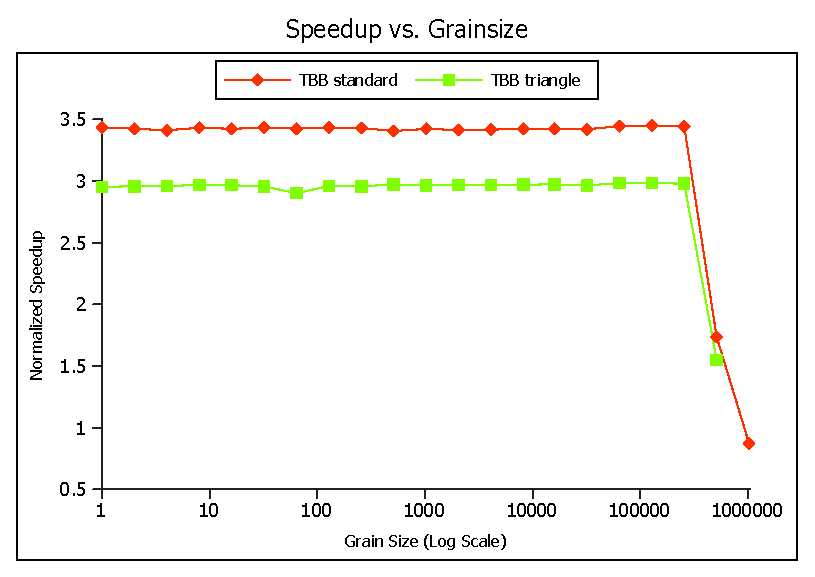
\includegraphics[width=.90\linewidth]{graph_tri_grain}

\subsection{Speedup vs. Number of Particles}

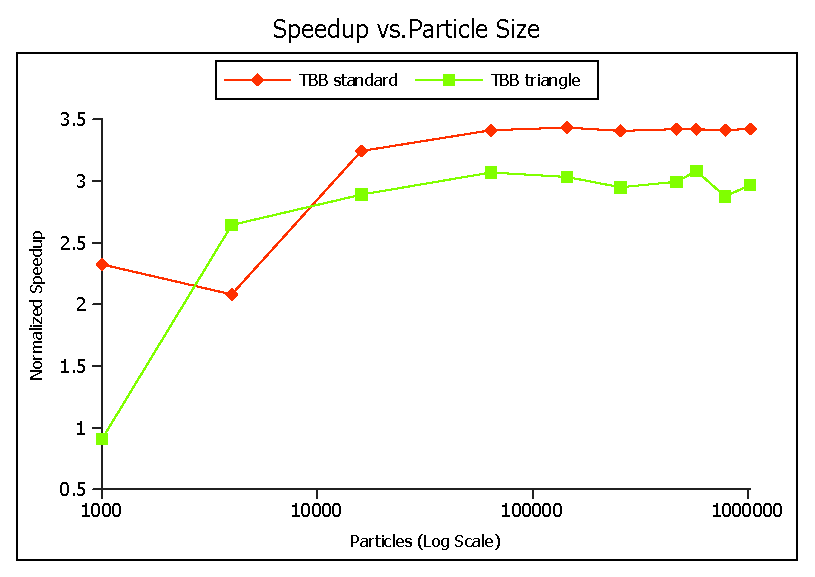
\includegraphics[width=.90\linewidth]{graph_tri_particle}

\subsection{Speedup vs. Number of Cores}

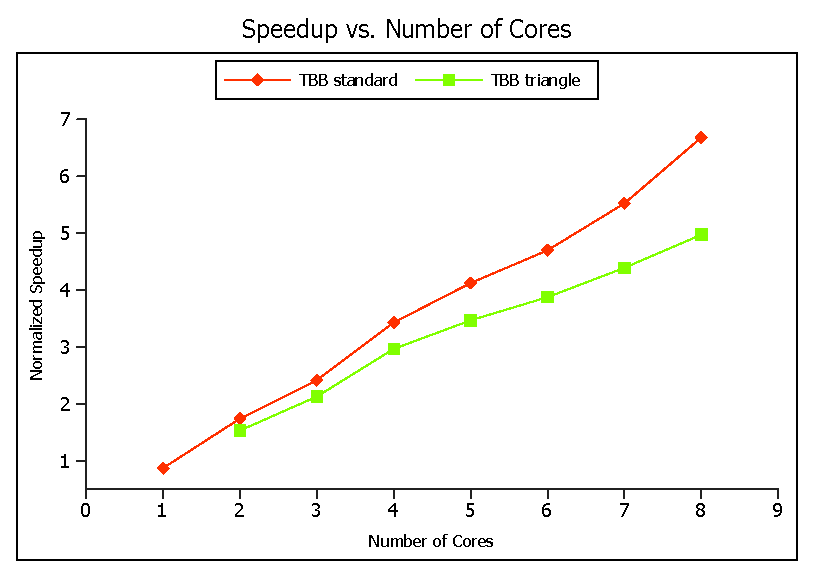
\includegraphics[width=.90\linewidth]{graph_tri_core}

\subsection{Speedup vs. Number of Clusters}

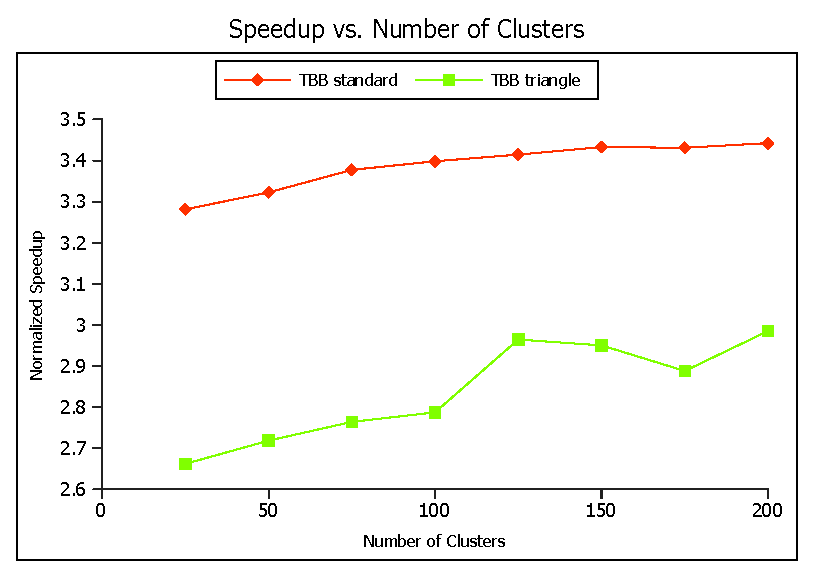
\includegraphics[width=.90\linewidth]{graph_tri_cluster}

\subsection{Brief Discussion of Results}

\section{Conclusion and Future Steps}

One natural extension to this work is to perform an in-depth analysis of the difference between the TBB and OpenMP code, such as by doing a thorough comparison of the assembly files produced by the TBB and OpenMP versions of the algorithm to see how they are using Intel's SIMD instructions differently. To go even further, the TBB and OpenMP implementations could be hand-tuned to use SSE vectorization, and the performance gains could be measured. Another extension would be to implement the k-means algorithm on a graphics card (for example, with CUDA) and compare its performance to the performances we achieved on the CPU. Some additional experiments would be to use different methods of packing the image data such as cohesive particle or cohesive image channels, to see which works best with the SSE vector instructions, or to use different color spaces or different distance functions on the input image.

\section{Appendix A - Source Code}
The source code that was used to perform these experiments is available at
\begin{verbatim}
https://cis534kmeans.googlecode.com/svn/trunk/
\end{verbatim}
via Subversion.

% needed in second column of first page if using \pubid
%\pubidadjcol

% trigger a \newpage just before the given reference
% number - used to balance the columns on the last page
% adjust value as needed - may need to be readjusted if
% the document is modified later
%\IEEEtriggeratref{8}
% The "triggered" command can be changed if desired:
%\IEEEtriggercmd{\enlargethispage{-5in}}
% references section
%\bibliographystyle{IEEEtran.bst}
%\bibliography{IEEEabrv,../bib/paper}
%\begin{thebibliography}{1}
%\bibitem{IEEEhowto:kopka}
%H.~Kopka and P.~W. Daly, \emph{A Guide to {\LaTeX}}, 3rd~ed. Harlow, England: Addison-Wesley, 1999.
%\end{thebibliography}

% You can push biographies down or up by placing
% a \vfill before or after them. The appropriate
% use of \vfill depends on what kind of text is
% on the last page and whether or not the columns
% are being equalized.

%\vfill

% Can be used to pull up biographies so that the bottom of the last one
% is flush with the other column.
%\enlargethispage{-5in}

\bibliographystyle{plain} % Please do not change the bib-style
\bibliography{writeup_bib} % Just the *.BIB filename

\end{document}
